\graphicspath{{figures/design/}}


			\chapter{Test Journal: Attached Flight}



\begin{table}[!h]
\begin{tabular}{l l}
\textbf{Test participants:} & Romain \& Raphael   \\
\textbf{Date:}  & 01/05-2017
\end{tabular}
\end{table}


			1st draft

	\section*{Purpose}
	
The purpose of the test is to experiment the hardware, software and controller of the rocker in a first aptempt of a stable flight. The objective is to approve the setling time.




	\section*{Test equipment and components}
	
\begin{table}[h]
	\centering
	\caption{List of measurement equipment and components}\label{tab_appendix:template}

	\begin{tabularx}{\textwidth}{lXXXX}
		Name 	\\ \toprule
		\rowcolor{lightGrey}
		Rocket body		\\
		Thruster	\\ 
		Camera 	\\
		Rope and poles \\ \rowcolor{lightGrey}
	\end{tabularx}
\end{table}




	\section*{Setup}
	
Measurement setup is seen on \autoref{fig:DCSetup} and photo \
%\begin{figure} [h]
%\centering
%
\includegraphics[width=0.6\linewidth]{figures/frontpage.jpg}
%\caption{Measurement setup.}
%\label{fig:DCSetup}
%\end{figure}

 The Rocket body is attached by two ground-fixed ropes on two opposite side position, around its center of pressure. The rocket has a maximum vertical movement of "unknown" meters.




	\section*{Method}
	
 The setup of the rocket will ennable a safe, for observers and the system, simulation of the rocket flight. The proper functionment of the controller is acheived if a stable movement of the ground-fixed rocket is observed.



	\section*{Raw data}

Photo of different positions + table of multiple test.

\begin{table}[htbp]
	\centering
	\caption{Measurment time of different set points.}
	\label{RPMData}
	\begin{tabular}{llll}
		Test & Flight duration{(}s{)} & Stabilisation starting point{(}ms{)} & Percentage  \\ \hline  \rowcolor{lightGrey}
		1     & 0              & 0             & 0                    \\
		2     & 0              & 0             & 0                    \\  \rowcolor{lightGrey}
		3     & 0              & 0             & 0                    \\ 
		4     & 0             & 0            & 0                    \\  \rowcolor{lightGrey}
		5     & 0             & 0            & 0                    \\
		6     & 0             & 0            & 0                    \\  \rowcolor{lightGrey}              
	\end{tabular}
\end{table}

	\section*{Data processing}

figure of mean time i guess
%\begin{figure}[htbp]
%	\centering
%	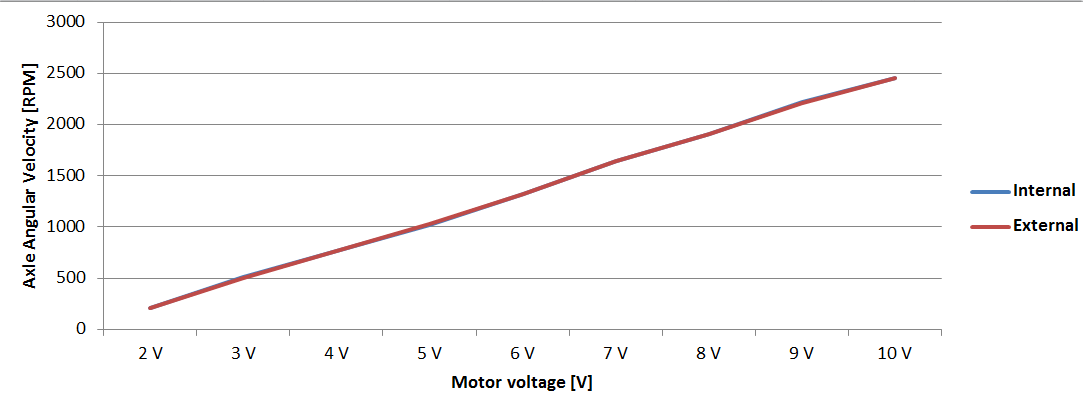
\includegraphics[width=\textwidth]{figures/appendix/Motor&GearTests/RPMTest}
%	\caption{Plot of RPM found for both tachometers}\label{fig:RPMTest}
%\end{figure}

	
The rocket becomes stable after a mean time of "unknown" secondes. This corresponds to a setling time of "unknown" secondes.
 
 
 

	\section*{Conclusion}

The rocket stability comes at an acceptable period of time after take-off. The hardware, software and controller are considered as successful, and the setling time fulfills the requirement.


